\documentclass[solution, letterpaper]{cs20inclass}
\usepackage{enumerate}
\usepackage{tikz}
\usepackage{pgf}
\usepackage{tikz}
\usepackage{hyperref}
\begin{document}
\header{20}{Monday, March 21, 2016}

\noindent Author: Erin Masatsugu% \\

\paragraph*{Executive Summary}
\begin{itemize}

\item Undirected Graphs: An undirected (or simple) graph $G = (V,E)$ consists of a set of vertices $V$ and a set of edges $E$, which are unordered pairs of \textit{distinct} vertices. To indicate that there is an edge $e$ between some vertices $a,b \in V$ we write $e = \{a,b\}\in E$. 

\item The degree of a vertex, denoted as $deg(v)$, is the number of edges incident to that vertex.

\item The Handshaking Lemma: In a simple graph $G = (V,E)$, the sum of degrees of all vertices is equal to twice the number of edges:
\begin{center}
$2|E| = \sum\limits_{v \in V}  deg(v)$
\end{center}
\item Graph Types:
\begin{itemize}
\item A graph is \emph{complete} if there is an edge between every pair of vertices; the complete graph on $n$ vertices is written $K_n$. 
\item A graph is \emph{bipartite} if we can separate its vertices into two sets, such that there are no edges between vertices of the same set. 
\item A graph is \emph{empty} if there are no edges. 
\end{itemize}

\item Undirected Graph Isomorphism: Two undirected graphs $G_1 = (V_1, E_1)$ and $G_2 = (V_2, E_2)$ are isomorphic if there is a bijective function $f: V_1 \rightarrow V_2$ such that
  $$\{a,b\} \in E_1 \Leftrightarrow \{f(a),f(b)\} \in E_2  $$

In other words, there is an edge between two vertices in $G$ if and only if there is an edge between their corresponding vertices in $H$. From this definition we can derive the following lemmas:
\begin{itemize}
\item Isomorphic graphs have the same number of edges.
\item Isomorphic graphs have the same number of vertices.
\item If $G$ and $H$ are isomorphic, then the degree of any vertex in $G$ must be equal to the degree of its corresponding vertex in $H$.
\end{itemize}
\end{itemize}

\paragraph*{In Class Problems}

\problem Are the two graphs below isomorphic? If no, explain why. If yes, for each vertex from the left graph give its corresponding vertex from the right one.
\begin{center}
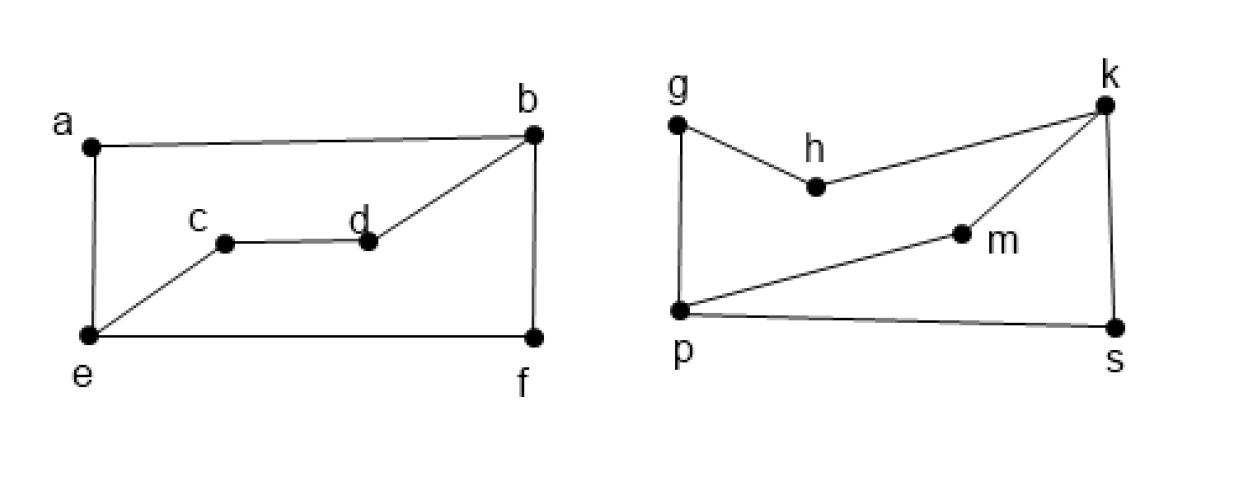
\includegraphics[scale=0.5]{isomorphisms.png}
\end{center}

\solution The graphs are isomorphic, and one possible bijection $f: $ LEFT $ \rightarrow $ RIGHT is:
\begin{itemize}
\item[] $ c \rightarrow g $
\item[] $ d \rightarrow h $
\item[] $ a \rightarrow m $
\item[] $ e \rightarrow p $
\item[] $ b \rightarrow k $
\item[] $ f \rightarrow s $
\end{itemize}

\problem Determine which among the four graphs pictured below are isomorphic. If two of these graphs are isomorphic, describe an isomorphism between them. If they are not, give a property that is preserved under isomorphism such that one graph has the property, but the other does not.
\begin{center}
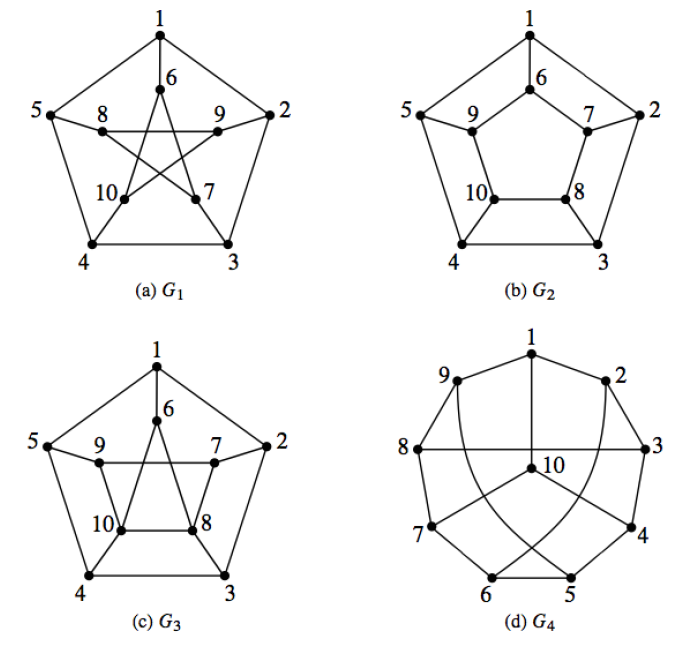
\includegraphics[scale=0.5]{isomorphisms_4.png}
\end{center}

\solution
\begin{itemize}
\item[] a and b are not isomorphisms because b has length-4 cycles while a does not.
\item[] a and c are not isomorphisms because c has nodes with degree 4 while a does not.
\item[] a and d are isomorphisms by the following translation: $a \rightarrow b: 1 \rightarrow 1, 2 \rightarrow 2, 3 \rightarrow 6, 4 \rightarrow 5, 5 \rightarrow 9, 6 \rightarrow 10, 7 \rightarrow 7, 8 \rightarrow 8, 9 \rightarrow 3, 10 \rightarrow 4$
\item[] b and c are not isomorphisms because c has nodes with degree 4 while b does not.
\item[] b and d are not isomorphisms because b has length-4 cycles while d does not.
\item[] c and d are not isomorphisms because c has nodes with degree 4 while d does not.
\end{itemize}

\problem Prove that if an undirected graph has more than two nodes and is bipartite, then it cannot be complete. Draw the undirected graph that has exactly two nodes and is both bipartite and complete.

\solution Proof by contradiction: Suppose there is an undirected graph with more than 2 nodes that is bipartite and also complete. If there is an edge between every pair of vertices (the definition of a complete graph), there are no two vertices which are not connected by an edge. Thus, the graph cannot be a bipartite graph. The undirected graph that has exactly 2 nodes and is both bipartite and complete is the graph with 2 nodes connected by an edge.

\problem (BONUS) Prove that any undirected graph with at least two vertices has at least two vertices of the same degree.

\begin{solution} Proof by contradiction: Suppose that there is a graph where every vertex has a different degree. In an $n$ vertex graph, vertices $1, 2, ..., n$ have degree $0, 1, ..., n-1$ (we do not allow self-loops). Vertex $n$ must be connected to every other vertex in the graph but vertex $1$ cannot be connected to any other vertex. Contradiction! This should be very familiar...
\end{solution}


\end{document}
